% Graphic for TeX using PGF
% Title: /home/afoek/Diagram1.dia
% Creator: Dia v0.97+git
% CreationDate: Wed Oct 28 10:44:29 2020
% For: afoek
% \usepackage{tikz}
% The following commands are not supported in PSTricks at present
% We define them conditionally, so when they are implemented,
% this pgf file will use them.
\ifx\du\undefined
  \newlength{\du}
\fi
\setlength{\du}{15\unitlength}
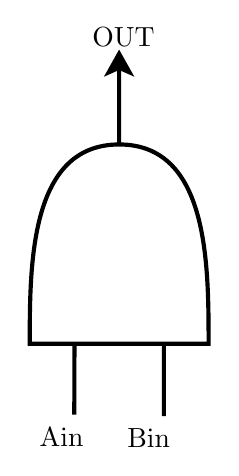
\begin{tikzpicture}[even odd rule]
\pgftransformxscale{1.000000}
\pgftransformyscale{-1.000000}
\definecolor{dialinecolor}{rgb}{0.000000, 0.000000, 0.000000}
\pgfsetstrokecolor{dialinecolor}
\pgfsetstrokeopacity{1.000000}
\definecolor{diafillcolor}{rgb}{1.000000, 1.000000, 1.000000}
\pgfsetfillcolor{diafillcolor}
\pgfsetfillopacity{1.000000}
\pgfsetlinewidth{0.100000\du}
\pgfsetdash{}{0pt}
\pgfsetbuttcap
\pgfsetmiterjoin
\pgfsetlinewidth{0.100000\du}
\pgfsetbuttcap
\pgfsetmiterjoin
\pgfsetdash{}{0pt}
\definecolor{diafillcolor}{rgb}{1.000000, 1.000000, 1.000000}
\pgfsetfillcolor{diafillcolor}
\pgfsetfillopacity{1.000000}
\definecolor{dialinecolor}{rgb}{0.000000, 0.000000, 0.000000}
\pgfsetstrokecolor{dialinecolor}
\pgfsetstrokeopacity{1.000000}
\pgfpathmoveto{\pgfpoint{-11.982500\du}{3.082446\du}}
\pgfpathcurveto{\pgfpoint{-9.828308\du}{3.082446\du}}{\pgfpoint{-9.828308\du}{5.963666\du}}{\pgfpoint{-9.828308\du}{7.884479\du}}
\pgfpathcurveto{\pgfpoint{-10.905404\du}{7.884479\du}}{\pgfpoint{-13.059596\du}{7.884479\du}}{\pgfpoint{-14.136692\du}{7.884479\du}}
\pgfpathcurveto{\pgfpoint{-14.136692\du}{5.963666\du}}{\pgfpoint{-14.136692\du}{3.082446\du}}{\pgfpoint{-11.982500\du}{3.082446\du}}
\pgfpathclose
\pgfusepath{fill,stroke}
\pgfsetlinewidth{0.010000\du}
\pgfsetbuttcap
\pgfsetmiterjoin
\pgfsetdash{}{0pt}
\definecolor{dialinecolor}{rgb}{0.000000, 0.000000, 0.000000}
\pgfsetstrokecolor{dialinecolor}
\pgfsetstrokeopacity{1.000000}
\pgfpathmoveto{\pgfpoint{-11.982500\du}{3.082446\du}}
\pgfpathcurveto{\pgfpoint{-9.828308\du}{3.082446\du}}{\pgfpoint{-9.828308\du}{5.963666\du}}{\pgfpoint{-9.828308\du}{7.884479\du}}
\pgfpathcurveto{\pgfpoint{-10.905404\du}{7.884479\du}}{\pgfpoint{-13.059596\du}{7.884479\du}}{\pgfpoint{-14.136692\du}{7.884479\du}}
\pgfpathcurveto{\pgfpoint{-14.136692\du}{5.963666\du}}{\pgfpoint{-14.136692\du}{3.082446\du}}{\pgfpoint{-11.982500\du}{3.082446\du}}
\pgfusepath{stroke}
\pgfsetlinewidth{0.100000\du}
\pgfsetdash{}{0pt}
\pgfsetbuttcap
\definecolor{dialinecolor}{rgb}{0.000000, 0.000000, 0.000000}
\pgfsetstrokecolor{dialinecolor}
\pgfsetstrokeopacity{1.000000}
\draw (-13.059596\du,7.884479\du)--(-13.063368\du,9.591405\du);
\pgfsetlinewidth{0.100000\du}
\pgfsetdash{}{0pt}
\pgfsetbuttcap
\definecolor{dialinecolor}{rgb}{0.000000, 0.000000, 0.000000}
\pgfsetstrokecolor{dialinecolor}
\pgfsetstrokeopacity{1.000000}
\draw (-10.905404\du,7.884479\du)--(-10.904279\du,9.625783\du);
% setfont left to latex
\definecolor{dialinecolor}{rgb}{0.000000, 0.000000, 0.000000}
\pgfsetstrokecolor{dialinecolor}
\pgfsetstrokeopacity{1.000000}
\definecolor{diafillcolor}{rgb}{0.000000, 0.000000, 0.000000}
\pgfsetfillcolor{diafillcolor}
\pgfsetfillopacity{1.000000}
\node[anchor=base west,inner sep=0pt,outer sep=0pt,color=dialinecolor] at (-13.897814\du,10.346991\du){Ain};
% setfont left to latex
\definecolor{dialinecolor}{rgb}{0.000000, 0.000000, 0.000000}
\pgfsetstrokecolor{dialinecolor}
\pgfsetstrokeopacity{1.000000}
\definecolor{diafillcolor}{rgb}{0.000000, 0.000000, 0.000000}
\pgfsetfillcolor{diafillcolor}
\pgfsetfillopacity{1.000000}
\node[anchor=base west,inner sep=0pt,outer sep=0pt,color=dialinecolor] at (-11.784556\du,10.384771\du){Bin};
\pgfsetlinewidth{0.100000\du}
\pgfsetdash{}{0pt}
\pgfsetbuttcap
\definecolor{dialinecolor}{rgb}{0.000000, 0.000000, 0.000000}
\pgfsetstrokecolor{dialinecolor}
\pgfsetstrokeopacity{1.000000}
\draw (-11.982500\du,3.082446\du)--(-11.983572\du,1.233239\du);
\pgfsetdash{}{0pt}
\pgfsetmiterjoin
\pgfsetbuttcap
\definecolor{diafillcolor}{rgb}{0.000000, 0.000000, 0.000000}
\pgfsetfillcolor{diafillcolor}
\pgfsetfillopacity{1.000000}
\fill (-11.983766\du,0.898866\du)--(-11.733507\du,1.344582\du)--(-11.983572\du,1.233239\du)--(-12.233507\du,1.344812\du)--cycle;
\definecolor{dialinecolor}{rgb}{0.000000, 0.000000, 0.000000}
\pgfsetstrokecolor{dialinecolor}
\pgfsetstrokeopacity{1.000000}
\draw (-11.983766\du,0.898866\du)--(-11.733507\du,1.344582\du)--(-11.983572\du,1.233239\du)--(-12.233507\du,1.344812\du)--cycle;
% setfont left to latex
\definecolor{dialinecolor}{rgb}{0.000000, 0.000000, 0.000000}
\pgfsetstrokecolor{dialinecolor}
\pgfsetstrokeopacity{1.000000}
\definecolor{diafillcolor}{rgb}{0.000000, 0.000000, 0.000000}
\pgfsetfillcolor{diafillcolor}
\pgfsetfillopacity{1.000000}
\node[anchor=base west,inner sep=0pt,outer sep=0pt,color=dialinecolor] at (-12.626410\du,0.724689\du){OUT};
\end{tikzpicture}
